\chapter{Spectral Energy Distribution towards Cl*\,1806-20}

% \mbox{HESS\,J1808-204} is a currently unidentified source of VHE gamma-rays towards stellar cluster \mbox{Cl*\,1806-20} and young magnetar \mbox{SGR\,1806-20} \citep{2018A&A...612A...1H}. The stellar cluster contains several energetic stars whose interacting winds accelerate cosmic rays to produce the gamma-ray emission towards \mbox{HESS\,J1808-204} \cite{2018A&A...612A..11H}. Alternatively, the SNR associated with \mbox{SGR\,1806-20} may be the origin of the gamma-ray emission. This section will investigate the origin of \mbox{HESS\,J1808-204} by modelling the multi-wavelength SED using \newsedprod (see \textcolor{red}{reference newsedprod intro})

% % Massive star clusters have been proposed as possible PeVatron candidates (see \textcolor{red}{reference pevatron discussion}), where interacting stellar winds accelerate cosmic rays up to $\PeV$ energies \citep{2019NatAs...3..561A}.

% \section{Cl* 1806-20}

% C1* 1806-20 is estimated to be located between $6-9~\kpc$; the distance used from heron is based on distance to containing magnetar at $8.7~\kpc$ \citep{2008MNRAS.386L..23B}. As well as containing four Wolf Rayet Stars, four OB type stars and the most luminous and massive blue variable star to data, LBV 1806-20; C1* 1806-20 also contains soft gamma repeater SGR 1806-20.
% \par~\par
% SGR 1806-20 is a magnetar, a type of neutron stars with extreme magnetic fields up to $10^{13}-10^{15}~\si{\gauss}$. SGR 1806-20 is most famous for the gamma-ray burst on the 27th December 2004 with luminosity reaching up to $10^{47}~\ergspersecond$  \citep{2005Natur.434.1098H}. To appreciate how large the luminosity is, the measured luminosity of HESS J1808-204 in photon energy range ($0.2-10~\TeV$) is $L_\text{VHE} = 1.6\times 10^{34} (\frac{d}{2})^2 ~\ergspersecond$ \citep{2008MNRAS.386L..23B}. The average x-ray luminosity towards this source is of order $10^{35}~\ergspersecond$. Based on the proper motion from infra-red observations and the that the magnetar originated from the stellar cluster at distance $8.7~\kpc$, the age of SGR 1806-204 is $650\pm 300~\si{yr}$ \citep{2012ApJ...761...76T}.
% \par ~ \par
% Located to the galactic north west of HESS J1808-204 lies SNR G10.0-0.3, a non-thermal radio nebula. It has been noted that SNR G10.0-0.3 has approximately the same intrinsic size as HESS J1808-204, $\ang{0.10}$. If SNR G10.0-0.3 is located at the same distance as HESS J1808-204, $8.7~\kpc$, the size of the radio nebula is $15.1~\kpc$. Assuming that SNR G10.0-0.3 is linked to the $650~\si{yr}$ magnetar, the SNR can be assumed to be the Sedov Taylor Phase (starting at $100~\si{yr}$). The radius of a SNR is this phase is estimated by \cite{2008ARA&A..46...89R}:
% \begin{align}
% 	R_\text{SNR}&=0.31E_{51}^{\frac{1}{5}}\qty(\frac{\mu}{1.4})^{-\frac{1}{5}} n_0^{-\frac{1}{5}}t_\text{yr}^{\frac{2}{5}}\quad\pc
% \end{align}
% where $E_{51}$ is the injected energy normalised to $10^{51}~\ergs$, $\mu$ is the mean mass per particle (assumed to be $1.4$), $n_0$ is the ambient gas density and $t_\text{yr}$ is the age of the SNR. Assuming an ambient gas density of $n_0=1~\centimeterminusthree$, the extent of the SNR linked to magnetar SGR 1806-20 to be $4.1_{-0.9}^{+0.7}~\pc$. This is quite different to the expected extent of $15.1~\kpc$, suggesting that SNR G10.0-0.3 is not linked to the magnetar inside C1* 1806-20. For a SNR aged $650~\si{yr}$ to have extent of $\ang{0.1}$ at distance $8.7~\kpc$, the ambient medium is required to have a density of $0.0015~\centimeterminusthree$. The above calculations assume that the supernova remnant is isolated. If SNR G10.0-0.3 is connected to C1* 1806-20 then it is possible that the combined stellar winds of surrounding massive stars may affect the evolution of the supernova remnant linked to SGR 1806-20.
% \par~\par
% It has been noted that the surrounding non-thermal radio nebula G10.0-0.3 peaks around luminous blue variable LBV 1806-20. With HESS J1806-204 similar extent and orientation to the nebula, it suggests a more likely connection to the luminous blue variable rather than the magnetar \colorbox{red}{Reference Molecular Paper here}
% \par~\par.
% Towards this cluster also lies two Fermi sources; 3FGL J1809.2-2016c and Fermi J1808.2-2029. 3FGL J1809.2-2016c and Fermi J1808.2-2029 are located towards the same region in the sky but the former is a point source object while Fermi J1808.2-209 is a circular extended source \citep{2016ApJ...827...41Y}.  Fermi J1808.2-2029 is believed to be located $4.7~kpc$ away with angular separation from HESS J1808-204 to be $\ang{0.35}$. In study by \cite{2016ApJ...827...41Y} the source of emission from fermi J1808.2-2019 is either the hadronic interaction between the SNR and nearby molecular clouds and (or a combination of) leptonic interactions with stellar winds from the cluster.


% \section{Gas Studies Towards HESS J1808-204}

% \begin{table}
% 	\centering
% 	\begin{tabular}{|c|c|c|c|c|c|c|}
% 		\hline
% 		& & \multicolumn{3}{|c|}{Distance ($\kpc$)} & \multicolumn{2}{|c|}{Density ($\centimeterminusthree$)} \\
% 		\hline
% 		Cloud & $v_\text{lsr}$ ($\kmpersec$) & Near & Far & Assumed & $\ce{^{12}CO(1-0)}$ & $\ce{^{13}CO(1-0)}$ \\
% 		\hline
% 		MC-16 & $-12.5$ & & & $4.5$ & $280$ & $18$ \\
% 		MC 13A & $12.5$ & $1.7$ & $15.1$ & $15.1$ & $140$ & $11$ \\
% 		MC 13B & $17$ & $2.2$ & $14.5$ & $4.5$ & $400$ & $38$ \\
% 		MC 24 & $24.5$ & $3.0$ & $13.8$ & $3.0$ & $310$ & $24$ \\
% 		MC 30 & $29.5$ & $3.5$ & $13.2$ & $3.5$ & $640$ & $28$ \\
% 		MC 44 & $43$ & $4.5$ & $12.3$ & $4.5$ & $150$ & $6.4$ \\
% 		MC 73 & $77$ & $5.7$ & $9.6$ & $8.7$ & $130$ & $14$ \\
% 		\hline
% 	\end{tabular}
% 	\caption{Density of CO gas towards HESS J1808-20 as found by \colorbox{red}{Reference Molecular Paper Here}}
% 	\label{tab:cluster_CO_density}
% \end{table}

% \begin{table}
% 	\centering
% 	\begin{tabular}{|c|c|c|c|c|c|c|}
% 		\hline
% 		& & \multicolumn{3}{|c|}{Distance ($\kpc$)} & \multicolumn{2}{|c|}{Density ($\centimeterminusthree$)} \\
% 		\hline
% 		Cloud & $v_\text{lsr}$ ($\kmpersec$) & Near & Far & Assumed & $\ce{^{12}CO(1-0)}$ & $\ce{^{13}CO(1-0)}$ \\
% 		\hline
% 		MC-16 & $-12.5$ & & & $4.5$ & $253$ & $18$ \\
% 		MC 13A & $12.5$ & $1.7$ & $15.1$ & $68$ & $140$ & $11$ \\
% 		MC 13B & $17$ & $2.2$ & $14.5$ & $246$ & $400$ & $38$ \\
% 		MC 24 & $24.5$ & $3.0$ & $13.8$ & $202$ & $310$ & $24$ \\
% 		MC 30 & $29.5$ & $3.5$ & $13.2$ & $220$ & $640$ & $28$ \\
% 		MC 44 & $43$ & $4.5$ & $12.3$ & $4.5$ & $94$ & $6.4$ \\
% 		MC 73 & $77$ & $5.7$ & $9.6$ & $8.7$ & $81$ & $14$ \\
% 		\hline
% 	\end{tabular}
% 	\caption{Density of CO gas towards HESS J1808-20 as found by \colorbox{red}{Reference Molecular Paper Here}}
% 	\label{tab:cluster_CO_density2}
% \end{table}

% \begin{table}
% 	\centering
% 	\begin{tabular}{|cccccc|}
% 		\hline
% 		Cloud & $B$ ($\si{\micro G}$) & $\tau_\text{sync}$ ($\times 10^3~\si{yr}$) & $R_\text{sync}$ ($\pc$) & $R_{10~\TeV}$ ($\pc$) & $R_{50~\TeV}$ ($\pc$) \\
% 		\hline 
% 		MC-16 & 10 & 13 & 66 & 15 & 22 \\
% 		MC 13A & 6 & 32 & 116 & 17 & 25 \\
% 		MC 13B & 12 & 8 & 50 & 14 & 21 \\
% 		MC 24 & 10 & 11 & 60 & 14 & 22 \\
% 		MC 30 & 16 & 4 & 34 & 13 & 19 \\
% 		MC 44 & 6 & 30 & 110 & 16 & 24 \\
% 		MC 73 & 6 & 36 & 123 & 16 & 25 \\
% 		\hline
% 	\end{tabular}
% 	\caption{The magnetic field strength of individual clouds calculated through Cruncher’s relationship. $\tau_\text{sync}$ represents the time it takes for electrons of $10~\TeV$ to lose all their energy through synchrotron cooling; the distance that these electrons diffuse in this time is given by $R_\text{sync}$. $R_{10~\TeV}$ and $R_{50~\TeV}$ is the distance that $10~\TeV$ and $50~\TeV$ electrons travel in $650~\si{yr}$ respectively. \colorbox{red}{Reference Molecular Paper Here}}
% 	\label{tab:sgr_diffusion_and_B}
% \end{table}


% Stars that are densely packed, as in stellar clusters, tend to blow out a bubble in the interstellar medium. Towards HESS J1808-204 nine components of molecular clouds has been noted by \cite{2004A&A...419..191C} in $\ce{^{12}CO(1-0)}$ and $\ce{^{13}CO(1-0)}$ gas data. A summary of these clouds as found by \colorbox{red}{Reference Molecular Paper here} is shown in table \ref{tab:cluster_CO_density}. Spatial correlation  between MC 73 and HESS J1808-20 was noted. This may indicate a connection between the gamma-ray emission observed from this region and this molecular cloud. It has been suggested by other studies that MC -16 is related to C1* 1806-20.
% \par~\par
% The parameters of cloud MC 73 will be considered while modelling the spectral energy distribution towards HESS J1808-204. For this reason densities of $14~\centimeterminusthree$ and $144~\centimeterminusthree$ (corresponding to the density of $\ce{^{13}CO(1-0)}$ and total $\ce{CO(1-0)}$ respectively) will be considered. The magnetic field can be obtained through Crutchers Relationship \citep{Crutcher_1999} (see Eq.~\ref{eq:ISM_crutchers}).

% \section{Single Zone Modelling towards HESS J1808-204}


% This work considers two possible scenarios to explain the gamma-ray emission towards HESS J1808-204. The first scenario is the continuous particle injection by the combined stellar winds from C1* 1806-20. The alternative is the sudden release of cosmic rays from the supernova remnant that occurred due to the creation of SGR 1806-20. HESS j1808-20 spectral energy distribution follows a simple power low ($\dv{N}{E}\propto E^{-\Gamma}$) with index $\Gamma=2.3\pm 0.2_\text{stat}\pm 0.3_\text{sys}$ and photon flux normalisation $2.9 \times 10^{-13}~\si{ph\per\centi\meter\squared\per\second\per\tera\electronvolt}$ \citep{2018A&A...612A..11H}.

% \subsection{Spectral Energy Distribution}

% The spectral energy distribution of objects towards HESS J1808-20 is shown in figure \ref{hess_j1808_20_spectra}. It is interesting to note that data measured by Fermi for 3DFGL J1809.20-2016c appears to follow the HESS data of HESS J1808-20. This may indicate that these two sources are connected and will be examined in this research. HESS  J1808-20 spectral energy distribution follows a simple power low ($\dv{N}{E}\propto E^{-\Gamma}$) with index $\Gamma=2.3\pm 0.2_\text{stat}\pm 0.3_\text{sys}$ and photon flux normalisation $2.9 \times 10^{-13}~\si{ph\per\centi\meter\squared\per\second\per\tera\electronvolt}$ \citep{2018A&A...612A..11H}.

% \subsection{Old and Continuous Source}

% \begin{figure}[p]
% 	% To include a figure from a file named example.*
% 	% Allowable file formats are eps or ps if compiling using latex
% 	% or pdf, png, jpg if compiling using pdflatex
% 	\begin{subfigure}[b]{0.9\columnwidth}
% 		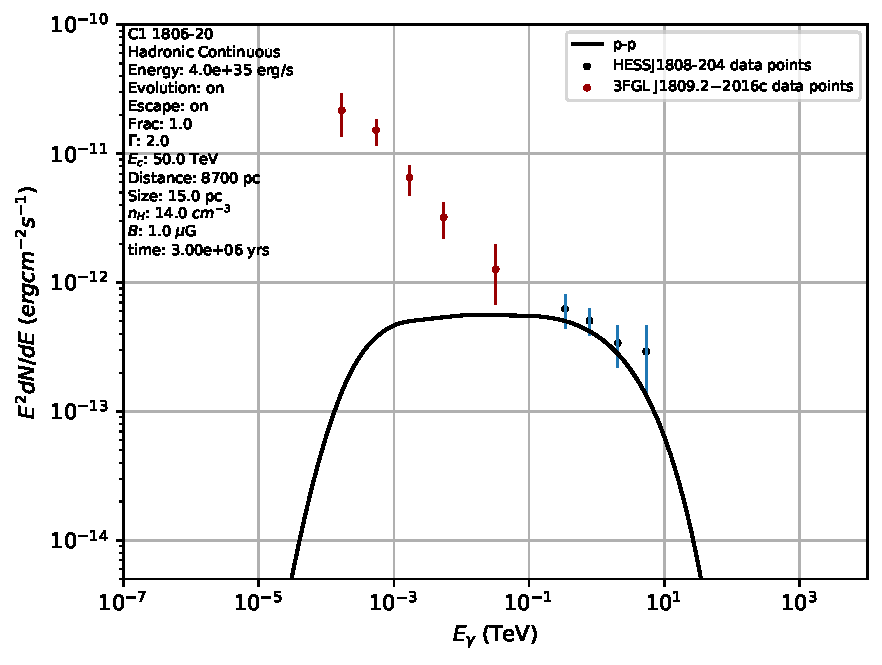
\includegraphics[width=\textwidth]{A5_HESS_J1808_204/Images/hadronic_continuous_cluster.pdf}
% 	\end{subfigure}
	
% 	\begin{subfigure}[b]{0.9\columnwidth}
% 		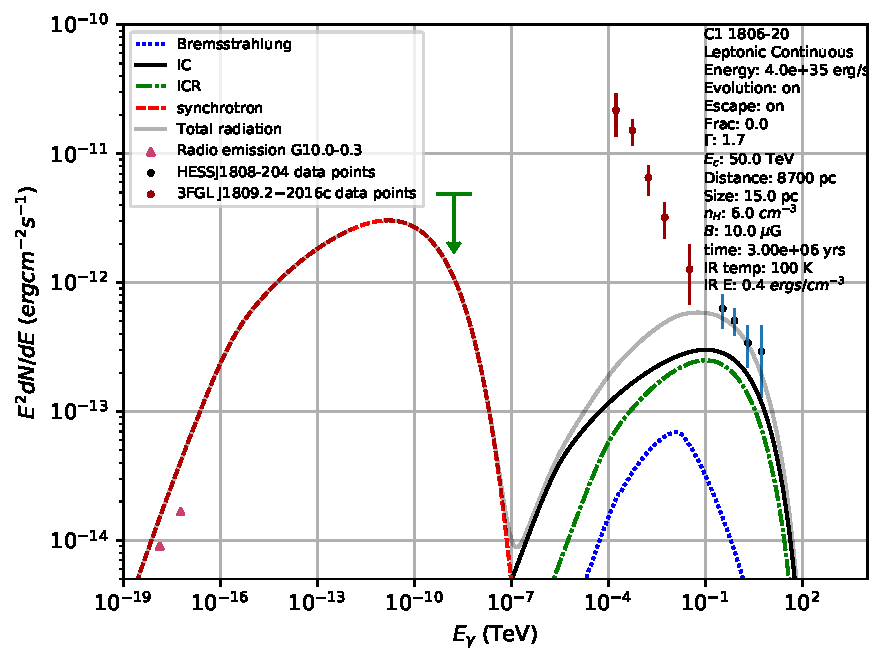
\includegraphics[width=\textwidth]{A5_HESS_J1808_204/Images/leptonic_continuous_cluster.pdf}
% 	\end{subfigure}
% 	\caption{Spectral Energy Distribution replication of HESS J1808-204 with combined stellar winds from super-massive stars as source of high energy particles. (\textit{top}) A purely hadronic scenario where observed gamma radiation is from proton-proton interactions. (\textit{bottom}) A purely leptonic scenario where observed gamma radiation comes from synchrotron (red dashed line), bremsstrahlung (blue dotted line) and IC interactions (green dashed lined for IR photons and solid black line for CMB photons). The total SED is shown in the transparent grey line.}
% 	\label{fig:continuous_cluster_SEDS}
% \end{figure}

% The particles constantly being injected into the surrounding medium around HESS J1808-20 allows gamma-rays to be emitted. Massive stars exist for over $1\times 10^6~\si{yr}$; the presence of the magnetar suggests that one of these old stars went supernova. Assuming that the predecessor of the magnetar is a O-type, the same type as stars contained within the cluster, this suggests the age of the system to be within range $0.1-10$ million years. Research into this system suggests that the age of C1* 1806-20 is between $3-4.5$ million years \citep{2005ApJ...622L..49F}.
% \par~\par
% The predicted spectral energy distribution of an old and continuous source can be shown in figure \ref{fig:continuous_cluster_SEDS}. High energy particles (both protons and electrons) are continuously injected into a molecular could with density $14~\centimeterminusthree$. The spectra of the high energy particles is assumed to be an exponential cutoff power law with $\dv{N}{E}\propto E^{-\Gamma}\exp(E/E_c)$. It has been estimated that stellar wind luminosity of a single massive can be as high as $10^{36}-10^{39}~\ergspersecond$ \citep{2018JKAS...51...37S}. The required energy budgets of both hadronic and leptonic scenarios, of order $10^{35}~\ergspersecond$, is well underneath this limit. Therefore an old and continuous source, such as the combined stellar winds of stellar cluster C1* 1806-20, as the origin of high energy gamma rays from HESS J1808-20 cannot be rejected.
% \par~\par
% It is interesting to note that for a purely leptonic scenario, the radio emission from G10.0-0.3 can be replicated. But for both a hadronic and leptonic case, the emission of Fermi source 3FGL J1809.2-2016.c can not be simultaneously predicted with the \HESS data.

% \subsection{Young and Impulsive Source}

% \begin{figure}[p]
% 	% To include a figure from a file named example.*
% 	% Allowable file formats are eps or ps if compiling using latex
% 	% or pdf, png, jpg if compiling using pdflatex
% 	\begin{subfigure}[b]{0.9\columnwidth}
% 		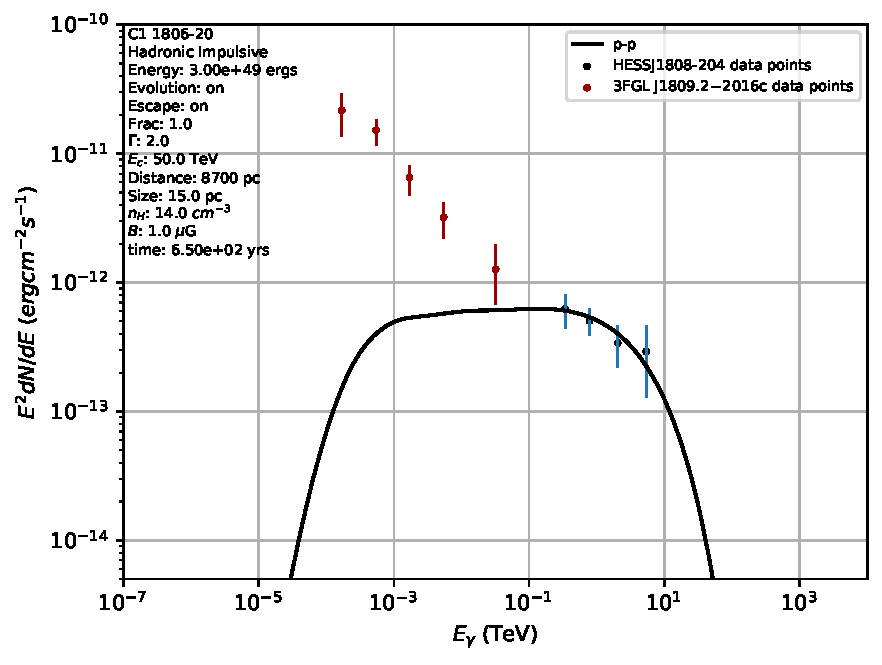
\includegraphics[width=\textwidth]{A5_HESS_J1808_204/Images/hadronic_impulsive_cluster.pdf}
% 	\end{subfigure}
	
% 	\begin{subfigure}[b]{0.9\columnwidth}
% 		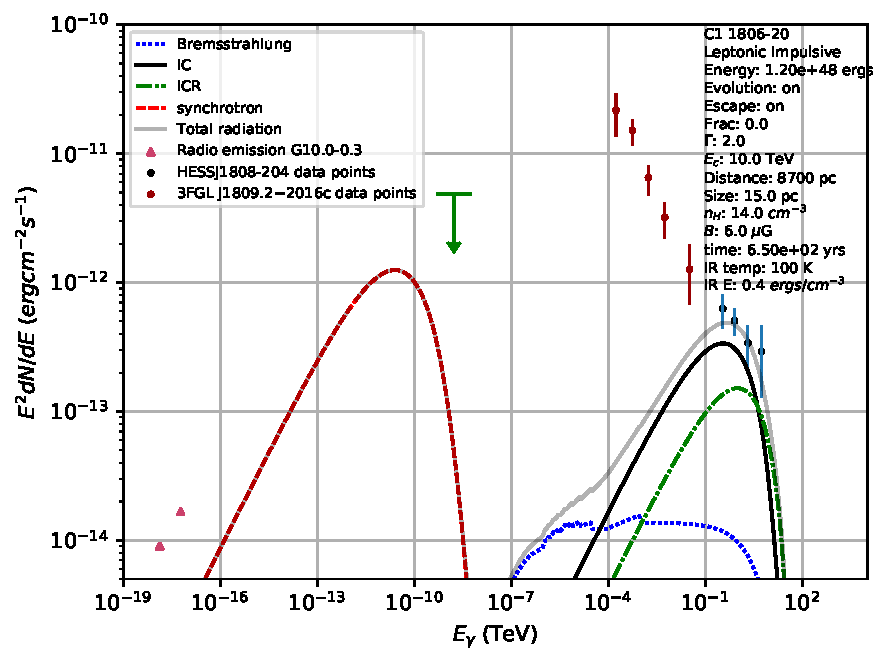
\includegraphics[width=\textwidth]{A5_HESS_J1808_204/Images/leptonic_impulsive_cluster.pdf}
% 	\end{subfigure}
% 	\caption{Spectral Energy Distribution replication of HESS J1808-204 with SNR related to SGR 1806-20 as source of high energy particles. (\textit{top}) A purely hadronic scenario where observed gamma radiation is from proton-proton interactions. (\textit{bottom}) A purely leptonic scenario where observed gamma radiation comes from synchrotron (red dashed line), bremsstrahlung (blue dotted line) and IC interactions (green dashed lined for IR photons and solid black line for CMB photons). The total SED is shown in the transparent grey line.}
% 	\label{fig:impulsive_cluster_SEDS}
% \end{figure}

% The presence of a magnetar inside C1* 1806-20 indicated that sometime in the past (approximately $650~\si{yr}$), a supernova occurred. This supernova remnant will impulsively release $10^{50}~\ergs$ of cosmic rays (approximately $10^{48}~\ergs$ partitioned to leptons) into the surrounding medium. The cosmic rays are then allowed to interact with the surrounding medium forming gamma-rays.
% \par~\par
% The results of the spectral energy distribution modelling can be seen in figure \ref*{fig:impulsive_cluster_SEDS}. Similarly to an old and continuous source, particles are injected into the interstellar medium with an exponential cutoff power-law ($\dv{N}{E}\propto E^{-\Gamma}\exp{E/E_c}$). $3.0\times 10^{48}~\ergs$ of cosmic rays is required to reproduce the spectra as seen by \HESS towards HESS J1808-20. This is well underneath the $10^{50}~\ergs$ upper limit and allows for a fraction of release cosmic rays to escape. On the other hand $1.20\times 10^{48}~\ergs$ of electrons is required to reproduce the spectra of HESS J1808-20. This is just within the upper limit of $10^{48}$. The radio emission of G10.0-0.3 cannot be replication with a young but impulsive source. For both cases, the observed Fermi emission towards 3FGL J1809.2-2016c cannot be simultaneous predicted with the \HESS data.

% \subsection{Combination}

% The more probably case for HESS J1808-20 is a combination of the SNR linked to the SGR 1806-20 and the combined stellar winds. This research did not consider the interaction between the SNR and combined stellar winds; though other studies suggest that supernova within stellar clusters allow cosmic rays to be accelerated up to $\PeV$ energies \citep{2018AdSpR..62.2764B}. Stellar Clusters are considered to be a possible candidate for high energy particle acceleration.